\documentclass[11pt,a4paper,ngerman]{article}
\usepackage[bottom=2.5cm,top=2.5cm]{geometry} 
\usepackage{babel}
\usepackage[utf8]{inputenc} 
\usepackage[T1]{fontenc} 
\usepackage{ae} 
\usepackage{amssymb} 
\usepackage{amsmath} 
\usepackage{graphicx}
\usepackage{fancyhdr}
\usepackage{fancyref}
\usepackage{listings}
\usepackage{xcolor}
\usepackage{paralist}

\usepackage[pdftex, bookmarks=false, pdfstartview={FitH}, linkbordercolor=white]{hyperref}
\usepackage{fancyhdr}
\pagestyle{fancy}
\fancyhead[C]{Approximation Algorithms}
\fancyhead[L]{Exercise sheet 1}
\fancyhead[R]{SoSe 2012}
\fancyfoot{}
\fancyfoot[L]{}
\fancyfoot[C]{\thepage \hspace{1px} of \pageref{LastPage}}
\renewcommand{\footrulewidth}{0.5pt}
\renewcommand{\headrulewidth}{0.5pt}
\setlength{\parindent}{0pt} 
\setlength{\headheight}{15pt}

\date{}
\title{Max Wisniewski}
\author{Dozent : Panos Giannopoulos}

\newcommand{\claim}{\addtocounter{claims}{1} \bfseries Claim \arabic{claims}}
\newcommand{\proof}{\bfseries Proof}


\begin{document}

\lstset{language=Pascal, basicstyle=\ttfamily\fontsize{10pt}{10pt}\selectfont\upshape, commentstyle=\rmfamily\slshape, keywordstyle=\rmfamily\bfseries, breaklines=true, frame=single, xleftmargin=3mm, xrightmargin=3mm, tabsize=2}

\renewcommand{\figurename}{Figure}
\newcounter{claims}

\maketitle
\thispagestyle{fancy}

%% ------------------------------------------------------
%%                     Exercise 1
%% ------------------------------------------------------

\section*{Exercise 1}

Consider the 2-approximation algorithm for the cardinality (i.e. unweighted) Vertex Cover problem that is based on computing a Maximal Matching. What approximation factor does it give for the general weighted vertex cover problem, where the vertices have arbitrary positive weights?\\

\textbf{Solution:}\\
Because $\delta$ is a function which domain is the set of instances for the problem we might take any information from the graph we need. The general idea to estimate the approximation factor is, that on each edge from the Maximal Matching, there might stand the maximal value of all nodes.\\
Because at least one of these nodes has to be part of the Minimum Vertex Cover we consider the worst case. One of these nodes contains the smallest possible value, the other one has the biggest on.\\
Now the weight of the two nodes on the edges we took is $\frac{max+min}{min} = \frac{max}{min}+1$ times as large as the smallest posibility might be.\\
We sum up every node in the Maximal Matching and because we know we know each pair of the matching is at most $\frac{max}{min}+1$ times as large, we can use the destribution law to extract the factor 
$$
	\delta (G(V,E)) = \frac{\max (V)}{\min (V)} + 1.
$$

\begin{description}
\item{\claim} $|C| \leq \left( \frac{\max (V)}{\min (V)} + 1 \right) \cdot OPT$ and $C$ is a vertix cover. 
\item{\proof}\\
In lecture the Theorem was given without proof, that for a unweighted graph $\mathfrak{A}$'s returnvalue is a Vertex Cover. If the graph is weighted, this fact is not changed in any way, because the definition of Vertex Cover is independend of any weight. So this claim holds.\\

$|C| \leq \left( \frac{\max (V)}{\min (V)} + 1 \right) \cdot OPT$ holds, because for each edge we took, we sum up a value that is $\delta$ times larger, than any in the Minimum Vertix Cover. The proof that we do not have more edges in the maximal matching then we have nodes in the Minimum Vertix Cover is the only remaining one.\\
But if we have less nodes in the Vertex Cover than edges the Maximal Matching takes, we have at least one edge in the Maximal Matching with both nodes not containt in the Vertex Cover. But, in case we have no multiedges, this can't be a Vertex Cover.\\
\mbox{}\hfill $\square$

\pagebreak

\item{\claim} $ \left( \frac{\max (V)}{\min (V)} + 1 \right) \cdot OPT$ is a tight upper bound.
\item{\proof} \\Let $G_n$ be a family of graphs, s.t. \\$G_i(V_i,E_i) = (\{a_t \; | \; 0 \leq t \leq 2i \}, \{ \{a_t, a_{t+1 \mod 2i} \; | \; 0 \leq t \leq i \})$ \\and together with a weight function \\$w_i \; : \; V_i \rightarrow Q^+ \; , a_t \mapsto \frac{1}{2} \cdot \left( (1+(-1)^t) + (1+(-1)^t) \cdot c \right)$ with $c \in \mathbb{Q}^+$ for each $i \in \mathbb{N}$ is a graph of this family.\\

For each $G_i(V_i,E_i)$ the Maximal Matching will deliver a $C$ through the algorithm $\mathfrak{A}$ that will consist of every node ($C=V_i$). Our weight function returns only 2 values. Either $1$ or $c$. Therefore the minimum of all nodes is $1$ and the maximum is $c$. We have as many minimum values on hte nodes as we have maximum values and each was taken from the Maximal Matching. Therefore $obj_{VC} (G_i, C) = c\cdot i + i$ holds.\\

As we can easily see, the minimum vertex cover will take every other node, namly the nodes with the minimum values. With that every edge has exactly one node taken in the Minimum Vertex Cover. For this graph therefore $obj_{VC}(G_i, OPT) = i$ holds.\\

Now $|C| = \left( \frac{\max (V)}{\min (V)} + 1 \right) \cdot OPT$ holds, because
$$
\begin{array}{rcl}
	|C|	&=& c \cdot i + i\\
		&=& \left( \frac{c}{1} + 1 \right) \cdot i\\
		&=& \left( \frac{\max (V_i) }{ \min (V_i) }\right) \cdot OPT \text{ holds.}
\end{array}
$$
\mbox{} \hfill $\square$
\end{description} 

%%--------------------------------------------------
%%		Exercise 2
%% -------------------------------------------------

\section*{Exercise 2}
Consider the following greedy algorithm for carinality Vertex Cover:
\begin{itemize}
	\item Input : Graph $G(V,E)$
	\item $C := \emptyset$
	\item While $C$ is not a vertex cover of $G$
		\begin{itemize}
			\item let $u$ be the vertex incident to the most uncovered edges
			\item $C := C \cup \{ u \}$
		\end{itemize}
	\item return $C$
\end{itemize}
\begin{figure}[!b]
	\centering
	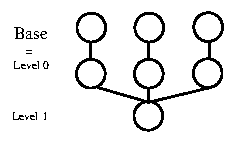
\includegraphics[width=1.75in]{ex2_anchor}
	\caption{Anchor of the graph familiy ($G_1$)}
	\label{fig:ex2:anchor}
\end{figure}

Is this a constant-factor approximation algorithm?\\

\textbf{Solution}\\
\begin{description}
	\item{\claim} The algorithm is not a constant-factor approximation algorithm.
	\item{\proof}


We construct a family of graphs that have a factor, dependend in the amount of vertices.\\
Let $G_n(V_n,E_n)$ be a family of graphs constructed as inductiv as followed:\\
$G_1(V_1,E_1)$ is a graph of the pairwise connected vertices and one vertex, that has a edge to one vertex of each pair. In figure \ref{fig:ex2:anchor} the graph is visualized.\\

Now for the Induction $G_i$ we take three graph of $G_{i-1}$. Further we add a number of new vertices to the graph and connect each of these vertices with each vertex in every baselayer in the three $G_{i-1}$ graphs, therefore the degree of these vertices will be $3^i$. The constructed graph looks like the example in figure \ref{fig:ex2:example} for the $G_2$.\\

The number of new vertices we will add must be as large as possible, but only that much, that our $3^i$ vertices in the baselevel will have at most the degree $3^i - 1$. From this we construct two formulas $\eta$ for the amount of vertices on level $k$ and $\Psi$ for all nodes (the pairs in the baselevel count as 1 per pair).


\begin{figure}[!b]
	\centering
	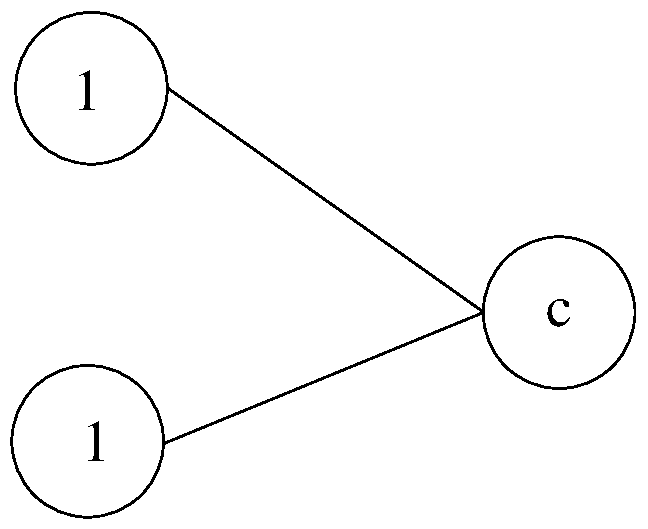
\includegraphics[width=\textwidth]{ex2_counter}
	\caption{Example for the graph $G_2$ of the family in exercise 2}
	\label{fig:ex2:example}
\end{figure}

$$
\begin{array}{rcl}
\eta & \; : \; & \mathbb{N}  \longrightarrow  \mathbb{N}\\
0 & \mapsto & 1\\
i & \mapsto & 3^i - \left( \underset{k=0}{\overset{i-1}{\sum}} \eta (k) \right) - 1 \quad , i>0 
\vspace{12pt}\\
\Psi & \; : \;&  \mathbb{N} \longrightarrow \mathbb{N}\\
i & \mapsto & 3^i + \underset{k=1}{\overset{i-1}{\sum}} 3^{k-1} \times \eta (i - k - 1)
\end{array}
$$

As one can easily see, the Vertex Cover must contain one vertex of each pair in the base level at least. Because every other edge is connected to the baselevel, the Minimum Vertex Cover will contain exactly one vertex (the one every edge is connected to) from each pair. So the OPT is $3^n$ for $G_n$.\\

The algorithm instead will take $\Psi (n)$ for $G_n$. This is, because we constructed the graph the way, that the vertices with the most uncovered edges are the one in the highest level. The base level will have at most one degree less, then the ones in the top level. After alle the toplevel vertices are taken for the Vertex Cover, the resulting graph will be three times $G_{n-1}$, because we could erase all taken nodes and edges connected to them, because the algorithm will no longer concern them as they all are covered.\\
The vertices we need for the vertex cover therefore will only be taken, after we took alle extra vertices from every level.\\

To proof this is not a constant-factor approximation we have to show, that $\frac{\Psi (n)}{ 3^n }$ is unbounded.
$$
\begin{array}{rcl}
\frac{\Psi(n)}{3^n} &=& 3^n + \underset{k=1}{\overset{n-1}{\sum}} 3^{k-1} \times \eta (n - k - 1) \cdot \frac{1}{3^n}\\
&=& 1 + \underset{k=1}{\overset{n-1}{\sum}} 3^{k - 1 - n} \times \eta (n - k - 1)
\end{array}
$$

For the result we must only concern ourselves with the sum. As we now through simple analysis these row diverge if the inner sequence does not converge against zero. Because we only sum up positive values the row would diverge against positive infinity.\\

\begin{description}
	\item{\claim} $\forall n > 0 : \eta (n) = 3^n - 3^{n-1}$
	\item{\proof} Induction over $n$\\
	\begin{description}
		\item{\bfseries I.A.} $n=1$\\
			$\eta (1) = 3^1 - 1 = 3^1 - 3^0$
		\item{\bfseries I.S.} $n \rightarrow n+1$\\
			$$
				\begin{array}{rcl}
					\eta(n+1) &=& 3^{n+1} - \left( \underset{k=0}{\overset{n}{\sum}} \eta (k) \right) - 1\\
						&\overset{\text{I.P.}}{=}& 3^{n+1} -  \left( \underset{k=0}{\overset{n}{\sum}} 3^k - 3^{k-1} \right) - 1\\
						&=& 3^{n+1} - 3^n - \left( \underset{k=1}{\overset{n-1}{\sum}} 3^k - 3^k \right)\\
						&=& 3^{n+1} - 3^n
				\end{array}
			$$
\mbox{}\hfill $\square$
	\end{description}
\end{description}

\pagebreak

If we take this claim into consideration
$$
\begin{array}{rcl}
\frac{\Psi(n)}{3^n} &=& 1 + \underset{k=1}{\overset{n-1}{\sum}} 3^{k - 1 - n} \cdot ( (3^{n-k-1} - 3^{n-k-2})\\
	&=& 1 + \underset{k=1}{\overset{n-1}{\sum}} 3^{k-1-n + n - k -1} - 3^{k - 1 - n + n - k -2}\\
	&=& 1 + \underset{k=1}{\overset{n-1}{\sum}} 3^{-2} - 3^{-3}\\
	&=& 1 + \underset{k=1}{\overset{n-1}{\sum}} \frac{2}{27}
\end{array}
$$
holds.

The inner sequence is a constant sequence and is never zero. Therefore the row does in fact diverge against positive infinity.\\

We proofed, that the approximation is not constant. \mbox{} \hfill $\square$

\end{description}



%% -------------------------------------------------------
%%			Exercise 3
%% ------------------------------------------------------

\section*{Exercise 3}
Consider the following approximation algorithm for the cardinality Vertex Cover problem: Find a depth first search tree $T$ in the given input graph $G$, and return the set $C$ of all the nonleaf vertices of $T$. Show that this is also a 2-approximation algorithm.\\

\textbf{Solution}\\
Let $\mathfrak{D}$ be the Algorithm described above. I assume the Graph $G$ is connected. Otherwise we can find a simple counterexample.

\begin{description}
	\item{\claim} The set $C$ returned by $\mathfrak{D}$ is a vertex cover.
	\item{\proof}

Let $G(V,E)$ be a valid instance for this problem and $T$ the DFS tree generated by $\mathfrak{D}$. A DFS tree in a Connected Graph visits all nodes. If not, there would exist an edge from a visited node to an unvisited one alongside the algorithm should have taken its path.\\

We now assume, there exists an edge $e=(i,j)\in E$ with $\{i , j\} \cap C = \emptyset$.\\
Every node, as stated above is visited, so $i,j$ may be either nonleaf vertices or leafs of the tree. If either of them would be a nonleaf vertex it would be in $C$. The only left possibility is, that both $i,j$ are leafs.\\
Let $i$ be the vertex visited first from the DFS algorithm w.l.o.g.. Then $j$ has to be a child of $i$, because the algorithm expects first all direct childs of $i$ before it returns to the parent of $i$. Because there exist an edge from $i$ to $j$ this edge is either taken in the DFS or there exists an edge from one of $i$ children to $j$. Either way $i$ can't be a leaf.\\

One can conclude, there is no edge, that has no vertex in the set $C$ and that implies, $C$ is a Vertex Cover.\\
\mbox{} \hfill $\square$  

\pagebreak

	\item{\claim} Let $G(V,E)$ be a graph and $T(V,E')$ be a spanning tree of $G$. \\If $I = \{v \in V \; | \; \deg_T (v) \geq 2\}$ is a Vertex Cover, then 
			$|I| \leq 2 \times OPT$ holds.
	\item{\proof}

Let $n =|V|$ the amount of vertices, $i = |I| = \left| \{ v \in V \; | \; \deg_T(v) \geq 2 \} \right|$ the amount of inner vertices.\\

Because every vertex except for the root in the tree has exactly one parent. So the amount of tree edges is $n-1$ and the amount of edges in between the nonleaf vertices is $i-1$.\\

Because of that fact the Vertex Cover has to be at least $\frac{i-1}{2}$ large as the amount of inner vertices $i$. So the optimal solution $OPT \geq \frac{i-1}{2}$.
Considering that
$$i \leq 2 \cdot \frac{i - 1}{2} + \frac{1}{2} \leq 2 \cdot OPT + \frac{1}{2}$$ holds, 
but both the optimal and the feasible solution of $\mathfrak{D}$ are natural Numbers, so the equation
$$
i \leq 2 \cdot OPT
$$
holds.\mbox{} \hfill $\square$

	\item{\claim} $\mathfrak{D}$ is a 2-approximation-algorithm.
	\item{\proof}

In claim 5 we had shown, that the DFS tree's inner vertices are a Vertex Cover. The DFS tree is a Spanning Tree, because it connects every vertex and is itself a tree. Together with claim 6 we now conclude, that the output $C$ of $\mathfrak{D}$ must assert
$$
|C| \leq 2 \cdot OPT.
$$
\mbox{}\hfill $\square$
\end{description}

\label{LastPage}

\end{document}